\chapter{Implementation Approach}
\label{chap:implementation}
\lhead{\emph{Implementation Approach}}
%The key question to be addressed in this chapter is: "How do I plan to achieve what I have outlined in the previous chapter".

%This chapter should comprise around 5000 words and specify your planned implementation approach. Again all sections below are suggestions and will vary significantly from project to project, the key element to be addressed is the core question of the chapter.

%\section{Architecture} \label{sec:Arch}
%Describe the architecture of the solution that you have in mind, including:
%\begin{itemize}
  %  \item Technologies involved (e.g., frameworks, programming language). 
 %   \item The hardware needed to develop the project (and to support at deployment stage)
%\end{itemize}

%Provide a high level view of the system you have in mind, including any package of classes, what is it responsible for and what other packages it communicates to. Provide a high level view of the database (or structure) needed to support the project, including what each table/document is responsible for and the hierarchy among them. You need to be as specific here as you can, why? Because this will aid you in identifying parts of the project you are vague on, this may be fine for some components but cause problems in term 2 for others. If you have hardware element in your project this is also where you provide a high level view of how these elements integrate into the project. So for a project that is cyber-physical you will have both a hardware and software architectural diagram. N.B. This is NOT a full system design but a high level overview of what you can credibly develop. This architecture should be informed by prototyping activity. 

%Some of the implementation focused projects may describe how do you envision tackling the functional requirements of your project via a set of use-cases. DFDs are also helpful here to understand elements of your project that may cause problems. You should describe the role of the different parts of the architecture of the solution, and the interaction among them.

\section{Risk Assessment}
With every project comes a risk. A risk is the possibility of losing something of value, an intentional interaction which can cause uncertainty. In any project there is a possibility that when progressing through the plan, that it becomes clear there is no feasible way the project can be implemented. This is also a possibility when implementing this idea. The technologies which are being used have been widely explored, proving their functionality. But there are no studies which show the migration of micro-services between devices. Although this is the case, there is no reason any issue which may rise can not be worked around or fixed. But, to be sure a risk analysis assessment must be carried out:

\textbf{ \underline {Uncertainty}} - \textit{Moderate}

Uncertainty is defined as an area of increased risk within a project. The level of uncertainty here is moderate. There are elements which are known to be fully functional, for example, we know that Raspberry Pi's are fully functioning single board computers. But, there is also the risk that the container might not sit correctly on the Raspberry Pi, which could lead to a whole re-work of this theory.

\textbf{\underline{Complexity}} - \textit{High}

Both complexity and uncertainty can be closely linked. Complexity aims to identify the level of difficulty attached to a project. For this project, the level of uncertainty is high. The reasoning for this is again, this is a new technique which has very little exploration, therefore, leaving the implementation to be widely unknown.

\pagebreak
\textbf{\underline{Size}} - \textit{Moderate}

The size and scale of a project is important to consider. The size of this project is moderate, the good thing about having this project implemented on Raspberry Pi's is scalability is never an issue. These edge devices can be moved, added and removed with little effort. Therefore, size would not be much of a risk factor. For this project, using just two SBC's keeps an element of simplicity.


\textbf{\underline{Project Management Level}} - \textit{High}

Project Management is extremely important. Project management involves planning, controlling and executing the tasks which are set out at the beginning of the project plan and ensure each stage is achieved as desired. 



%hese technologies, which enforces the possibility of failure.IFrom my research, there is very little to display that this would be a failure. The technologies are extremely scalable and flexible, which is exactly what is needed.dening ttify any potential risk precluding you from successfully complete your project. This section is really important and often neglected by students resulting in fatal risks occurring in some projects. Make sure to give this section the time it requires. Classify the risk according to their importance, possibility of arising and enumerate the decisions you can make to anticipate them or mitigate them (in case they finally arise). Table \ref{tab:ProjRisks} may help with this classification. This section should include your mitigation approach for any critical risks.

%\begin{table}[h]
%\centering
%\scriptsize
%\caption{Initial risk matrix}
%\begin{tabular}{|p{2cm}|p{2cm}|p{2cm}| p{2cm} |p{2cm}| p{2cm}|}
%\hline \bf Frequency/ Consequence & \bf 1-Rare & \bf 2-Remote & \bf 3-Occasional & \bf 4-Probable & \bf 5-Frequent\\ [10pt]

%\hline \bf 4-Fatal & \cellcolor{yellow!50} & \cellcolor{red!50} & %\cellcolor{red!50} & \cellcolor{red!50} &\cellcolor{red!50} \\ [10pt]

%\hline \bf 3-Critical &\cellcolor{green!50} & \cellcolor{yellow!50} & \cellcolor{yellow!50} & \cellcolor{red!50} &\cellcolor{red!50} \\ [10pt]

%\hline \bf 2-Major & \cellcolor{green!50} & \cellcolor{green!50} & \cellcolor{yellow!50} &\cellcolor{yellow!50} &\cellcolor{red!50} \\ [10pt]

%\hline \bf 1-Minor & \cellcolor{green!50} & \cellcolor{green!50} & \cellcolor{green!50} &\cellcolor{yellow!50} &\cellcolor{yellow!50} \\ %[10pt]
%\hline
%\end{tabular} \\
%\label{tab:ProjRisks}
%\end{table}

\section{Methodology}
%Describe your personal approach on how to tackle the different parts of this project, including:
%\begin{itemize}
 %   \item How to tackle the needed research to fulfill the background chapter. 
  %  \item How to set up your Computer Science skills to the project needs (e.g., describe your plan to learn any new technology involved on the project that you are not familiar with). 
   % \item What core project managing approach will you follow (e.g., Waterfall, Scrum, etc).
%\end{itemize}

There are many elements, needed to bring this idea to reality. One element which is hugely important and is the backbone for any project is the research. To ensure accurate and efficient information is provided, extensive research must be carried out. For the research of this project, it was important that all information was sourced from a variety of sources. These included books, ebooks, journals, wikis, blogs and whitepapers. 

The background research is needed to ensure this project will come together, but, as this is a project based on computer science subjects and technologies, there is more in-depth learning required. From the hardware to the software which will be used, there is some level of upskilling needed. This includes:

\textit{Raspberry Pi}

Learning the setup and functionality of a Raspberry Pi. This is a very important step as the Raspberry Pi backbone of this project. Setting up the SBC's is going to be the first step in the implementation phase. Because of this, knowing every aspect and detail required to ensure that this technology can be used to its highest potential for this project is essential. There are many many books and tutorials online to help with this process, which have been and will continue to be hugely beneficial throughout the implementation phase. 

\textit{Containers}

Containers are what this project is mainly focused on. Meaning, that extensive research needs to be taken on this element. As containers are a somewhat unknown technology and is not explored in my chosen course of study, the research and learning curve has been taken upon myself solely for this. With much information on containers and different types of containers and container orchestration tools, this element of the project will be an interesting and exciting one. 


Most of the other technologies involved are ones which have been studied over the last four years of studies in Cork Institute of Technology. Even though this is the case, due to any potential risk that could occur, it is important that research is continually carried out throughout both the research and implementation phases. This is mainly to ensure the project idea can be delivered to the highest ability. 


Every project requires management. For this project I researched some project life-cycle models to decide which would best be suited to this particular project. There are many life-cycle models which can be implemented for projects of this type. These include \textit{waterfall}, which is the oldest type of life-cycle used, it includes setting phases and not moving onto the next phase until the phase before is completely finished. Next, \textit{Agile}. This type of project life-cycle focuses on mainly software development, but can be used by project managers for all technology type of projects. The aim of the agile method is for the project manager to continually inspect and asses the workings of the team to ensure sufficient work and goals are being achieved. And finally, \textit{evolutionary} model. The evolutionary model is split into two main models, spiral and prototyping. The spiral model works alongside the prototyping model to mainly asses the risk which is attached to the different stages of the process. The prototyping model's main focus is to produce a fully functioning prototype for the project at hand. 

\vspace{5mm}
\textbf{\large Evolutionary Model}

The life-cycle model which is appropriate for this project is the evolutionary model. As previously discussed, this model can be used for projects which have a prototype aspect while also assessing the risks which are inevitable in a project. This project is heavily focused on developing a prototype. The evolutionary prototype model has five phases which work towards quick development of the prototype required. As seen in figure 4.1, these phases include communication, quick design, modeling quick design, construction of prototype and deployment, delivery and feedback.



\begin{figure}[ht]
    \centering
      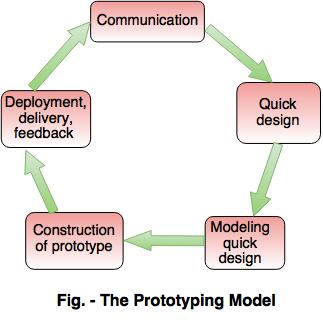
\includegraphics[width=0.65\textwidth]{Figures/PrototypeModel.jpg}
  \caption[prototype model]{Evolutionary Prototype Model \cite{Reference19}}
  \label{fig:Prototype Model}
\end{figure}

\vspace{5mm}

\begin{figure}
    \centering
     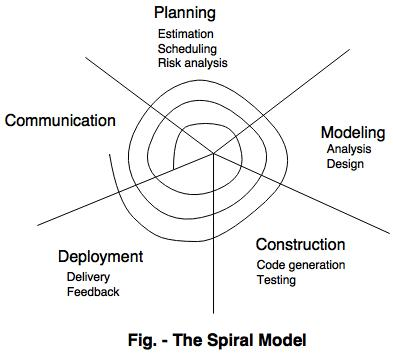
\includegraphics[width=0.65\textwidth]{Figures/SpiralModel.jpg}
  \caption[spiral model]{Evolutionary Spiral Model \cite{Reference19}}
 \label{fig:Spiral Model}
\end{figure}

\pagebreak

Not only are these phases used for the prototyping model, but they are also used for the spiral aspect of the evolutionary model. As seen in figure 4.2, the same phases are used to asses the risks which could potentially occur. 


\section{Implementation Plan Schedule}
%Come up with a schedule for the remaining time (including second semester), so as to describe how do you envision to achieve the implementation of your project by the end of semester 2. This plan SHOULD be ambitious but MUST be realistic and SHOULD be informed by early prototyping and MUST be discussed with your term 1 supervisor.

Throughout the implementation phase of this project, there will be a total of 200 hours expected to be invested. This level of commitment is needed for a project of this stature as there is a lot of additional research needed throughout. As seen from the risk assessment, there is a level of uncertainty involved with this project. I will break down the plan and time-line for the second phase of the project in a table:

\vspace{5mm}
\begin{tabular}{ |p{1cm}|p{6cm}| }
 \hline
 \multicolumn{2}{|c|}{Implementation Plan} \\
 \hline
 Week & Plan\\
 \hline
 1   & Install Operating System's on both Raspberry Pi's \\
 \hline
 2  &  Install Containers (Docker) on both Raspberry Pi's\\
 \hline
 3 & Troubleshoot any issues which may rise during installation process\\
 \hline
 4 & Install Kubernetes on both Containers\\
 \hline
 5 & Troubleshoot and resolve any issues which involve Kubernetes\\
 \hline
 6 & Install Virtual Machines on Kubernetes as Micro-services\\
 \hline
 7 & Test Virtual Machines and troubleshoot any issues\\
 \hline
 8 & Attempt migrating of microservices from one RP to the other \\
 \hline
 9 & Investigate and Troubleshoot issues which may occur. \\
 \hline
 10 & Investigate the aspect of transforming topology into an edge/fog environment \\
 \hline
 11 & Attempt to implement this type of architecture \\
 \hline
 12 & Review and Document all workings\\
\hline
\end{tabular}

\pagebreak
Having 12 weeks to implement the project in the second semester, I have set a goal of having one task to complete a week. These tasks are set with the mind set that they will take an estimated average of 16 hours each. 16 hours is a lot of time to allocate per week/per task but, from the research carried out in this phase of the project, it is clear every hour will be used to full advantage. Below is image 4.[], a Gantt chart of the estimated times I expect each task to take: 
\vspace{8mm}

\begin{figure}[ht]
    \centering
     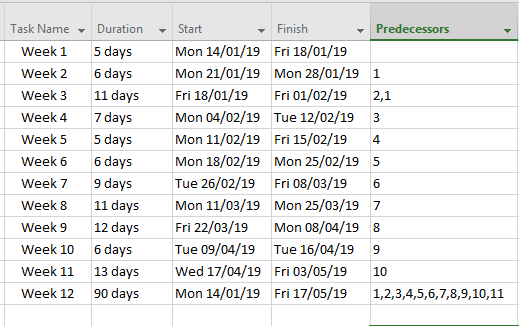
\includegraphics[width=0.95\textwidth]{Figures/ProjectPlan.PNG}
  \caption[Gantt chart Times]{Gantt Chart Times \cite{Reference19}}
 \label{fig:Gantt chart Times}
\end{figure}

\vspace{10mm}

Some of the tasks above can be seen to have shorter duration's than others. The reasoning behind this is to allow for some extra time to troubleshoot issues which may occur and potentially make any changes needed to improve the fore-coming prototype. Figure 4.4 shows the gantt chart layout for this project and how time will be spent during the implementation phase or second semester of this project. From January to May there is one continuous linked task which is set to write the required documentation for the implementation phase while ensuring weekly that tasks are being achieved. 
\pagebreak

\begin{figure}[ht]
    \centering
     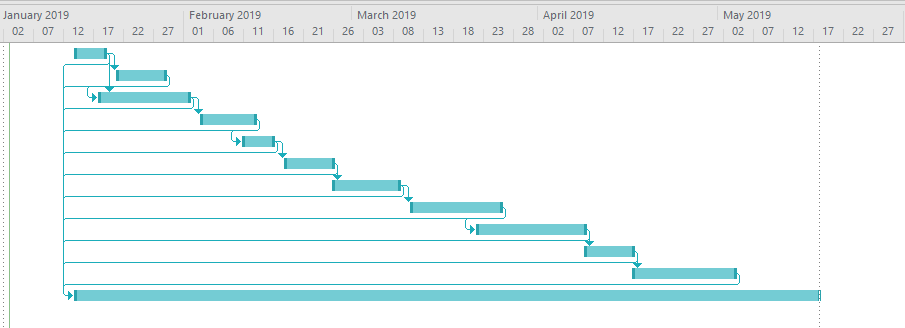
\includegraphics[width=1.0\textwidth, height=10cm]{Figures/GanttChart.PNG}
  \caption[Gantt Chart]{Gantt Chart \cite{Reference19}}
 \label{fig: Gantt Chart}
\end{figure}


\section{Evaluation}
%Come up with an evaluation plan that allows you to measure how much have you actually achieved the goals of your project. This again is a section that is often neglected where students loose marks. How do you plan to measure the output of your project? A binary it works/does not work is insufficient. You need to be able to quantify the success against both the functional requirements and the initial idea. These are not the same as you may meet all function requirements outlined but not solve the overall problem because you have failed to revisit these and update them with new information which you learn as you are developing the project.
Evaluating is essential to ensure that an accurate examination of the project is taken. The main aim of an evaluation is to analyze all aspects while assessing the outcome of the project. To achieve an effective project in both research and implementation, it is important to ask important questions:

\begin{enumerate}
    \item What was the purpose of the project?
    \item What is the expected outcome of this project?
    \item Who will this project benefit and why?
    \item Will this project be of use in future technologies?
    \item Are project targets being met and will they continue to be achieved?
    \item How will the project be assessed to ensure requirements are being met? 
\end{enumerate}

These being just some important questions which need to be answered. Project managers should gather information from an evaluation and use this information to determine the route to which the project takes. For this project, the evaluation would be based around the practicality of the migration of micro-services. The following questions need to be completed throughout this evaluation both before the implementation and during:

\begin{enumerate}
    \item Does the chosen container function on the Raspberry Pi?
    \item Will kubernetes run effectively on this container?
    \item Is it possible to install virtual machines on kubernetes?
    \item Will the migration of these micro-services be feasible?
    \item How will issues be resolved which may occur?
    \item Is it possible to share data other than microservices between the two Raspberry Pi's?
\end{enumerate}

Once these questions are repeatedly asked and answered throughout the course of the project, then understanding where the project direction is going will be much more clear. 

\section{Prototype}
%Although you do not have a fully functional project yet, you should show wireframes, snapshots or representation on how do you envision your project to look once the implementation phase has been completed. The nature of this section will vary significantly from project to project and can include anything from code snippets to snapshots of service deployments. Any prototyping you have done during the term should be summarized here that has not been captured in earlier sections. For example if you are planning to host your project using AWS in an EC2 instance you should have at least created a "hello world" setup to determine the basics, this probably should have been discussed in section \ref{sec:Arch}.
During the implementation phase of this project, I will aim to design a functioning prototype. This prototype will consist of the following aspects:
\begin{itemize}
    \item Two Raspberry Pi's
    
    These raspberry pi's will be used as the core compute systems. 
    
    \item Docker
    
    Docker, the container element of this project, will be installed and ran on the raspberry pi's. Here is where all functionality will occur.
    
    \item Kubernetes
    
    The orchestration tool for the containers, providing an overall view of the system.
    
    \item Virtual Machine
    
   Raspberry Pi's can be configured to have a Linux operating system to function. A virtual machine or machines, will be installed on the Raspberry Pi to show the functionality of micro-services.  
    
\end{itemize}

\pagebreak
As a general overview, figure 4.5 outlines the basic layers of this project:

\begin{figure}[ht]
    \centering
     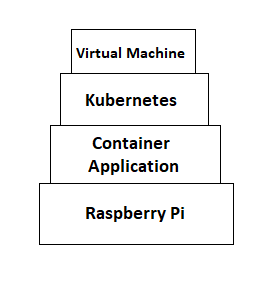
\includegraphics[width=0.45\textwidth, height=8cm]{Figures/Architecture.PNG}
  \caption[Architecture Layers]{Architecture Layers \cite{Reference19}}
 \label{fig:Architecture Layers}
\end{figure}

The prototype for this project will take some time to develop, as seen in the evaluation section. The final product will have the appearance of just two raspberry Pi's connected to a keyboard, mouse and monitor. From the outside appearing to be quite a simplistic prototype, the core of the raspberry pi's is where the technology lies to perform the function set out. 

The two Raspberry Pi's will be connected to a keyboard, mouse and monitor as shown:


\begin{figure}[ht]
    \centering
     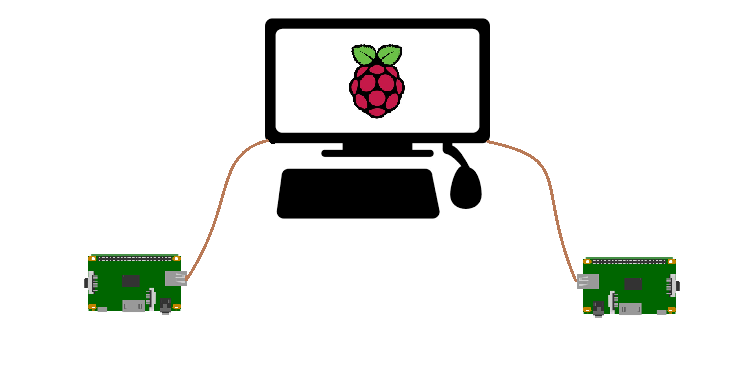
\includegraphics[width=1.0\textwidth,  height=8cm]{Figures/Topo.PNG}
  \caption[Topology]{Topology \cite{Reference19}}
 \label{fig:Topology}
\end{figure}


Once the Raspberry Pi's have been connected to a monitor, keyboard and mouse, each will be configured with an operating system. Raspbian is the operating system which the Raspb

Each Raspberry Pi will be configured with Docker. As previously discussed, Docker is the container engine being used for this project. Once Dock